\subsection{Tarefa 02}

\begin{comandoquestao}
    Objetivo. Analisar como a quantidade de épocas de treinamento influencia o desempenho da rede neural na aproximação da função seno. Observaremos como diferentes números de épocas afetam a convergência da perda e a qualidade das predições da rede.
\end{comandoquestao}

No presente treinamento, treinamos 4 redes neurais distintas. Todas tem a mesma 
características, mesmo modelo, mesmas funções de ativação nas camadas 
intermediárias (gelu) e mesma taxa de aprendizado. No entanto cada uma delas 
foi treinada com um número diferente de épocas. Vemos os resultados nas 
\cref{tarefa02:1000:predicoes,tarefa02:5000:predicoes,tarefa02:10000:predicoes,tarefa02:20000:predicoes}
 a seguir. Na \cref{tarefa02:figura:curvas} tem-se as curvas de erros durante o 
treinamento para as redes neurais. Na \cref{tarefa02:tabela:perdas} vemos as 
perdas para um mesmo conjunto de dados de teste referentes às diferentes redes 
neurais.


\begin{figure}[htb]
	\centering
	\begin{minipage}{0.45\textwidth}
	\centering
	\caption{Treinando com 1k épocas.}\label{tarefa02:1000:predicoes}
	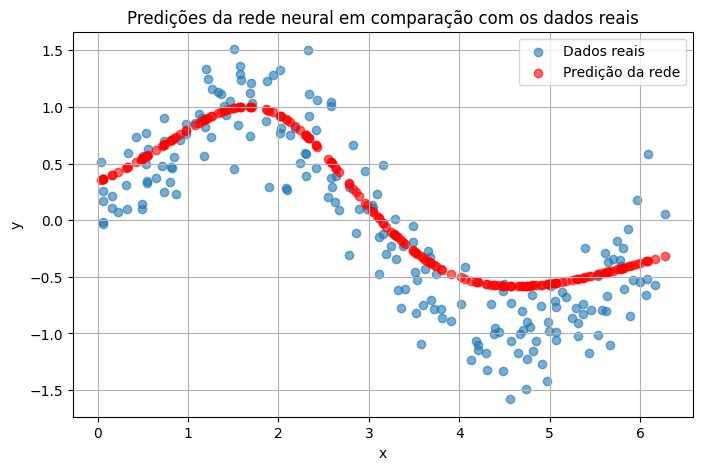
\includegraphics[width=\textwidth]{./0803_imgs/png-241110-154527304-12037654268696582542.png}
	%\legend{Fonte: Gerado peloComando da atividade}
	\end{minipage}
	\hfill
	\begin{minipage}{0.45\textwidth}
	\centering
	\caption{Treinando com 5k épocas.}\label{tarefa02:5000:predicoes}
	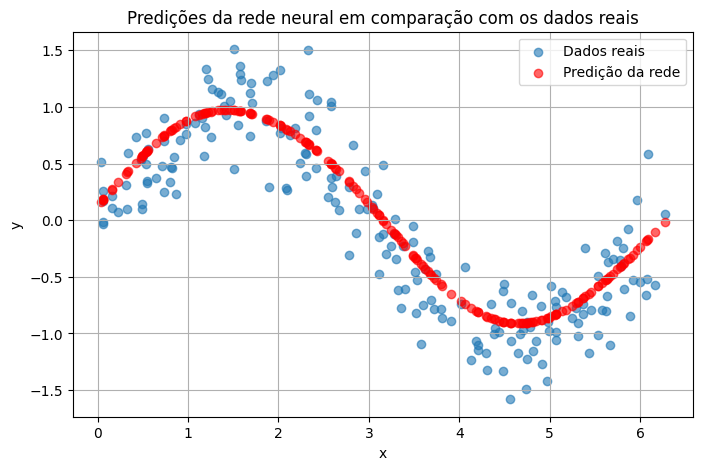
\includegraphics[width=\textwidth]{./0803_imgs/png-241110-154628196-17784737572676737911.png}
	%\legend{Fonte: \citeonline[p. 24]{araujo2012}}
	\end{minipage}
    \vspace{1Ex}
    \begin{minipage}{0.45\textwidth}
        \centering
        \caption{Treinando com 10k épocas.}\label{tarefa02:10000:predicoes}
        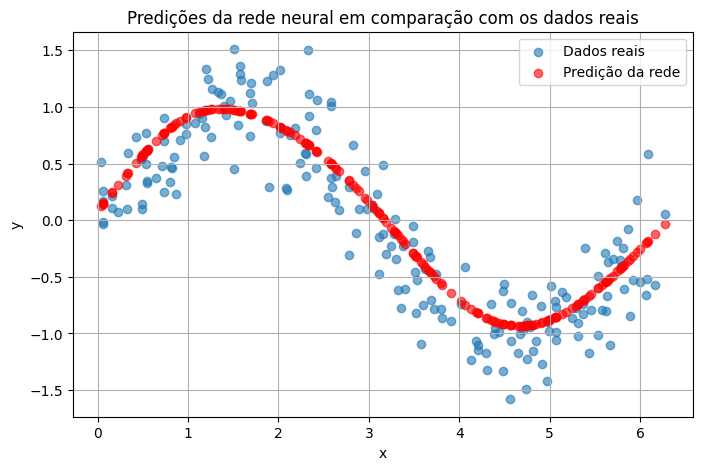
\includegraphics[width=\textwidth]{./0803_imgs/png-241110-154812342-18762265025268743.png}
        %\legend{Fonte: \citeonline[p. 24]{araujo2012}}
    \end{minipage}
	\hfill
	\begin{minipage}{0.45\textwidth}
	\centering
	\caption{Treinando com 20k épocas.}\label{tarefa02:20000:predicoes}
	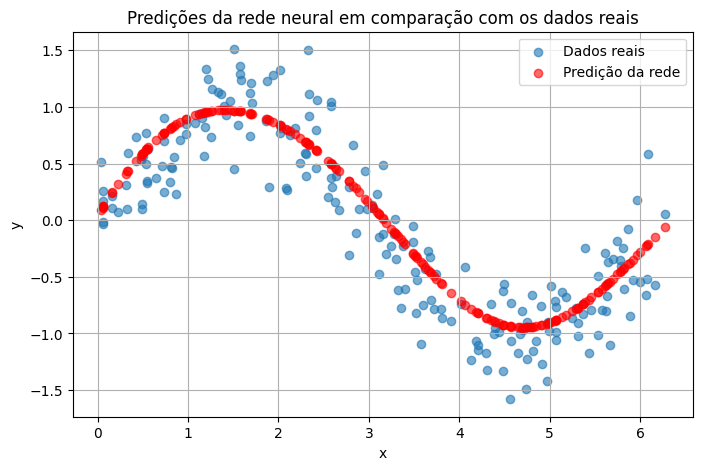
\includegraphics[width=\textwidth]{./0803_imgs/png-241110-155300412-9439382542521307108.png}
	%\legend{Fonte: \citeonline[p. 24]{araujo2012}}
	\end{minipage}
\end{figure}

\begin{figure}
	\centering
	\caption{Curvas de perdas durante o treinamento para as diferentes 
	redes}\label{tarefa02:figura:curvas}
	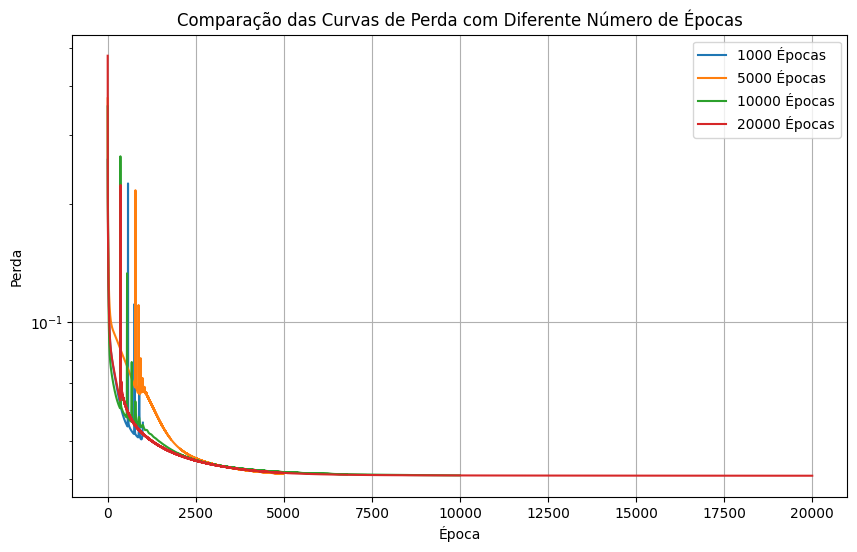
\includegraphics[width=0.7\linewidth]{./0803_imgs/png-241110-160937603-16503693892993531452.png}
\end{figure}

\begin{table}[htb]
	\caption{Perda de teste para as diferentes redes neurais}
	\centering
	\label{tarefa02:tabela:perdas}
\begin{tabular}{c | c}
	Rede Neural & Perda com dados de teste \\
	1k épocas  &  0.06468 \\
	5k épocas  &  0.04504 \\
	10k épocas &  0.04528 \\
	20k épocas &  0.04492
\end{tabular}
\end{table}

Observamos que a partir do treinamento com 5000 épocas as redes neurais tem 
erros muito próximos e uma maior quantidade de treinamento não faz uma 
diferença significativa na capacidade de predição das redes. O caso especial 
que podemos apontar é a rede treinada com a apenas 1000 épocas, a qual tem um 
erro bem acima das demais e aparentemente reflete um caso de ``underfitting''. 
Uma observação secundária é que esta rede 'Gelu' treinada por 1000 épocas, tem 
uma capacidade de previsão parecida com a rede treinada utilizando sigmóide 
como a função de ativação (\cref{tarefa01:simoide:predicoes})
